% Source: graduate-coursework/Sp26/CSCE763/Course_Assignments/HW3/HW3_CSCE_763_solutions.tex

\documentclass[border=4pt]{standalone}
\usepackage{amsmath}
\usepackage{amssymb}
\usepackage{graphicx}
\usepackage{tikz}
\usepackage{xcolor}
\usetikzlibrary{shapes.geometric, arrows.meta, positioning, patterns, calc}

\definecolor{USC_Garnet}{HTML}{73000A}
\definecolor{USC_Sandstorm}{HTML}{FFF2E3}
\definecolor{USC_Black90}{HTML}{363636}
\definecolor{USC_Black70}{HTML}{5C5C5C}
\definecolor{USC_Black50}{HTML}{A2A2A2}
\definecolor{USC_Black10}{HTML}{ECECEC}
\definecolor{USC_Honeycomb}{HTML}{65780B}
\definecolor{USC_Atlantic}{HTML}{466A9F}
\definecolor{USC_Congaree}{HTML}{1F414D}
\definecolor{USC_Rose}{HTML}{CC2E40}
\definecolor{USC_Grass}{HTML}{CED318}
\definecolor{USC_Horseshoe}{HTML}{65780B}
\definecolor{outputbg}{RGB}{245,245,245}

\begin{document}
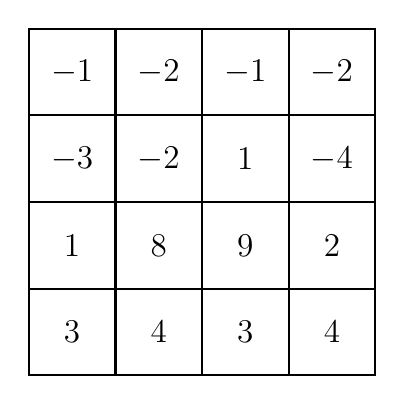
\begin{tikzpicture}[
  cell/.style={minimum size=1.1cm, draw=black, thick, fill=white, font=\large\bfseries},
]
\node[cell] at (0,3.3) {$-1$};
\node[cell] at (1.1,3.3) {$-2$};
\node[cell] at (2.2,3.3) {$-1$};
\node[cell] at (3.3,3.3) {$-2$};

\node[cell] at (0,2.2) {$-3$};
\node[cell] at (1.1,2.2) {$-2$};
\node[cell] at (2.2,2.2) {$1$};
\node[cell] at (3.3,2.2) {$-4$};

\node[cell] at (0,1.1) {$1$};
\node[cell] at (1.1,1.1) {$8$};
\node[cell] at (2.2,1.1) {$9$};
\node[cell] at (3.3,1.1) {$2$};

\node[cell] at (0,0) {$3$};
\node[cell] at (1.1,0) {$4$};
\node[cell] at (2.2,0) {$3$};
\node[cell] at (3.3,0) {$4$};
\end{tikzpicture}
\end{document}
